\documentclass{article}
\usepackage[utf8]{inputenc}
\usepackage{graphicx, graphics, float}
\usepackage[a4paper, total={6in, 9in}]{geometry}
\usepackage[spanish]{babel}
\usepackage{subcaption}
\title{Haz Una Línea\\
\large Memoria DS - Práctica 3}
\author{Andrés Merlo Trujillo\\ Sergio Hervás Cobo\\ Javier Serrano Lucas\\ Ricardo Molina Rodríguez}

\begin{document}
\date{Abril 2022}
\maketitle
\section{Introducción}
En esta práctica se ha realizado una serie de pruebas para comprobar el funcionamiento correcto de
ciertas funcionalidades y métodos de la aplicación realizada en la Práctica 2 (Haz Una Línea). Se han implementado
tests de unidad que comprobarán si la ejecución de un método de una clase produce el resultado
esperado y tests de widgets que buscarán la existencia de algún elemento que permita verificar su buen funcionamiento.

En total se han realido 4 tests de widgets y 8 de unidad que explicaremos a continuación en los siguientes apartados.


\section{Tests de unidad}
\begin{itemize}
\item \textbf{El volumen de la música debería cambiar a 0:} Clase: Música.

Para este test se ha comprobado que el volumen de la música es 0 cuando se llama a "setSonido".
De esta forma se comprobará si de verdad el volumen del sonido cambia dentro de dicho método cuando el usuario aprieta el botón del cambio de volumen.

Se dará como correcto si el valor del volumen que almacena la clase pasa a ser 0.

\item \textbf{El volumen de la música debería cambiar a 1:} Clase: Música.

Para este test se ha comprobado que el volumen de la música es 1 cuando se llama a "setSonido" dos veces.
De esta forma se comprobará si de verdad el volumen del sonido cambia dentro de dicho método cuando el usuario aprieta dos veces el botón del cambio de volumen.

El test dará resultado correcto si el valor del volumen que almacena la clase acaba siendo 1.

\item \textbf{La pieza no se debe mover en los bordes del tablero:} Clase: Pieza

Este test verifica si al mover una pieza que está en el borde del tablero en esa misma dirección, esta permanece en el mismo sitio sin salirse del tablero. Se hace
comprobando cada pieza que puede existir en el tablero y mirando si sus coordenadas están dentro de las del tablero.

El test se dará como correcto si todas las piezas no se salen del tablero tanto por la izquierda como por la derecha.

\item \textbf{La bomba explota: }Clase: PiezaBomba.

Este test se encarga de comprobar que las piezas bombas al detonar eliminan los bloques colindantes a los propios bloques de la pieza bomba.
Se dará como correcto si los bloques del tablero de alrededor de la bomba y los de la propia pieza bomba son nulos.

\item \textbf{La pieza esta en el suelo:} Clase: Pieza.

Este test comprueba que la pieza al bajarla se encuentre en el suelo del tablero y no se haya pasado más de la cuenta.

Se dará como correcto este test si la pieza no se sale de los límites del tablero y se encuentra en el suelo.

\item \textbf{Todas las piezas creadas son distintas:} Clase: Factoria

Este test comprueba que el algoritmo usado en la factoria para obtener las piezas es consistente. Se ha hecho un algoritmo tipo ``saco'', en el que un tipo de pieza no vuelve a salir hasta que no salgan las demás. Por tanto este test se encarga de comprobar que las 7 primeras piezas son distintas, como es de esperar.

Se dará como correcto el test si al sacar el mismo número de piezas que las pasadas a la factoría al final son todas distintas.

\item \textbf{La pieza detecta colision con otra de abajo:} Clase: Pieza

Este test se encarga de comprobar que al poner una pieza encima de otra no la atraviese y detecte correctamente la colisión.

El test sacará un resultado satisfactorio si al bajar una pieza, hay otra debajo (los bloques debajo del tablero no son nulos).

\item \textbf{Cuando se forman 10 bloques horizontales se destruye una linea:} Clase: Tablero

Este test consiste en colocar 10 bloques (en este caso 5 cubos) y comprobar que al hacer la línea (2 en esta ocasión) se eliminan del tablero. Se ha realizado una modificación
en la clase Tablero para poder instanciarlo, ya que al ser un State, la clase es privada por defecto.

El test se dará como correcto cuando todas las casillas del tablero sean null, debido a que hemos colocado 5 pieza de tipo cubo, haciendo dos líneas perfectas sin ningún bloque sobrante.
\end{itemize}

\begin{figure}[H]
      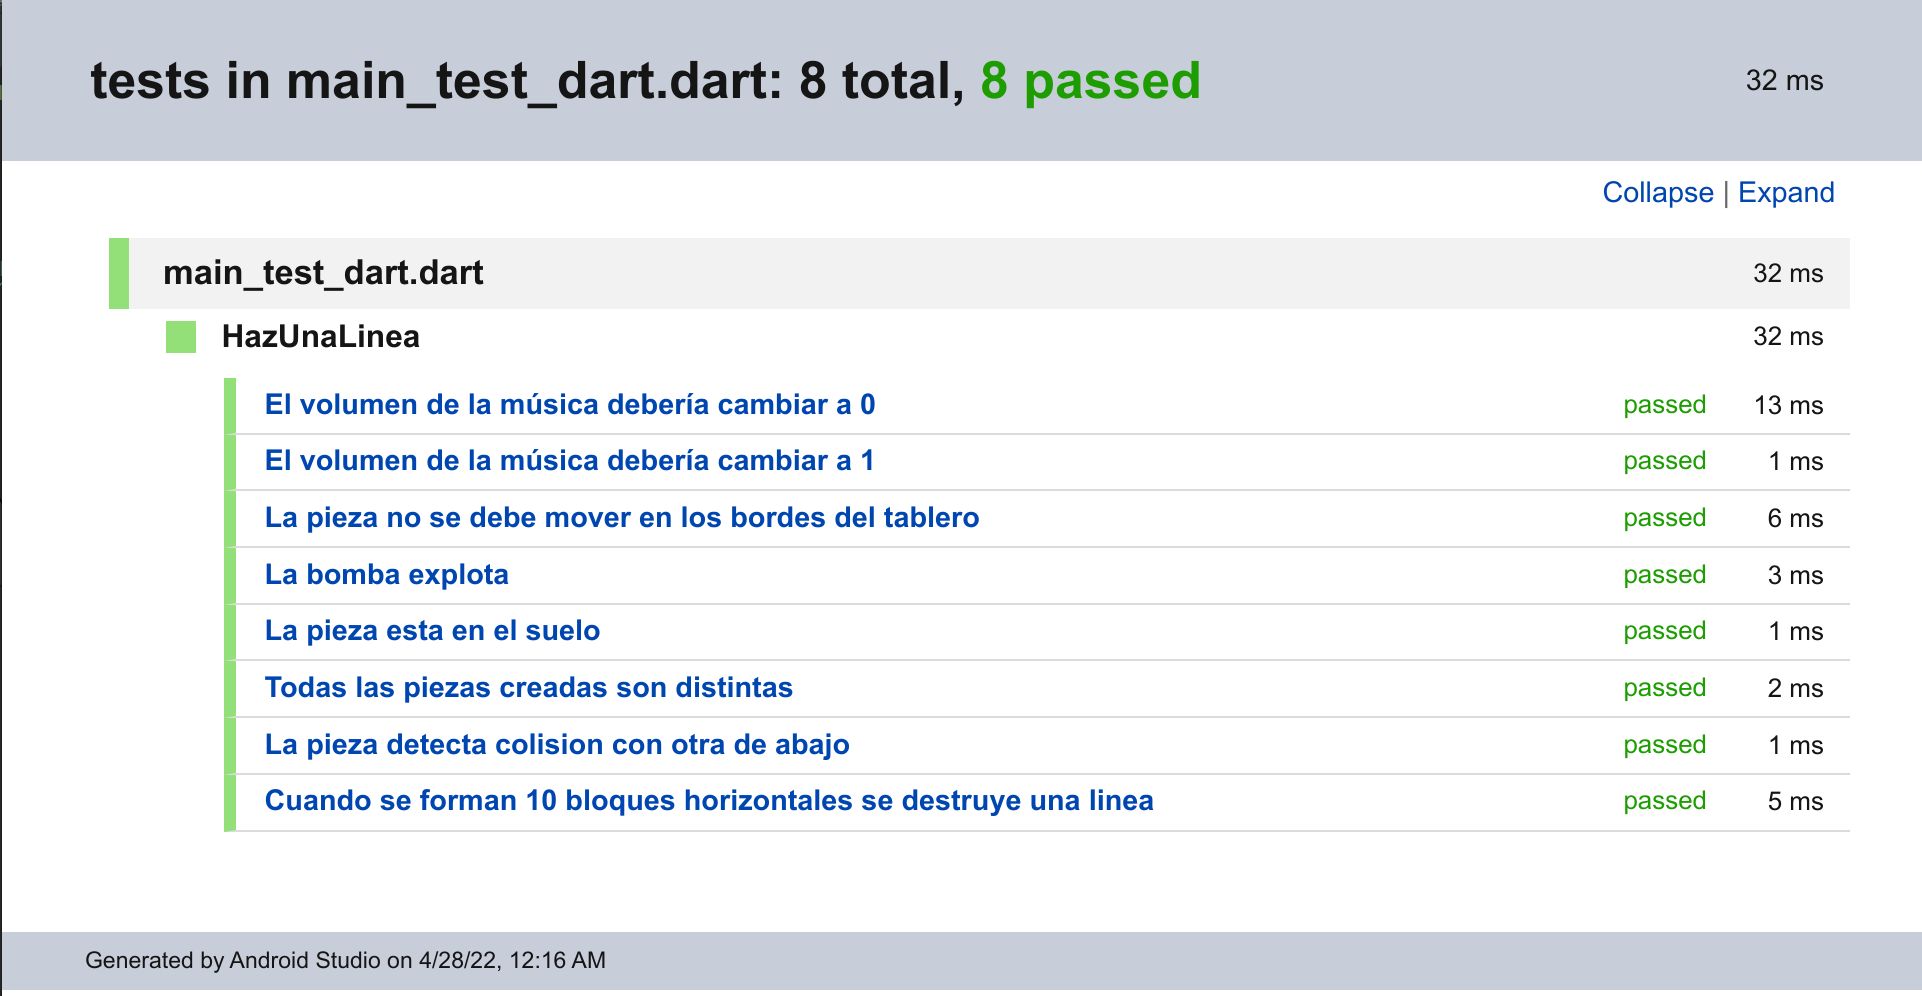
\includegraphics[width=\textwidth]{imagenes/dart_test.png}
      \caption{Resultado de los tests de unidad}
\end{figure}

\newpage

\section{Tests de Widgets}
\begin{itemize}
\item \textbf{Cambio de icono al apagar/encender la musica:} Clase: Música.

Se comprobará si el icono del altavoz se alterna al apretarlo para cambiar el volumen de la música.
Se hace apretando el botón de iniciar partida, luego el icono de pause y luego el botón para cambiar el volumen.

Se dará como correcto este test si al pulsar el botón el icono del mismo cambia al otro que se espera.

\item \textbf{Aparece la pantalla de Game Over:} Clase: GameOver.

Se comprueba si al pasar un tiempo, el juego termina por la llegada de las piezas a la parte
superior del tablero.

Se dará como correcto este test si al perder la partida aparece la pantalla de Game Over.

\item \textbf{Al salir de la partida desde el menú de pausa regresa al menú principal:} Clase: Pausa

Se verifica si al pulsar el botón de salir en la pantalla Pause, se saca de la pila el widget del tablero y del Pause y vuelve a la pantalla de inicio.

Se dará como correcto este test cuando al salir desde el menú de pausa se desapilen todas las pantallas y vuelva a aparecer la pantalla de inicio.

\item \textbf{Al reservar pieza, esta aparece en la pantalla: }Clase: Tablero.

Se comprueba si al pulsar "Guardar" por primera vez, la pieza actual pasa a ser una pieza reservada mediante
un find.ByKey (previamente se ha tenido que poner una key a la pieza reservada para poder
encontrarla)

Se dará como correcto este test cuando al reservar la primera pieza en la partida, esta salga en el recuadro asignado.

\end{itemize}

\begin{figure}[H]
      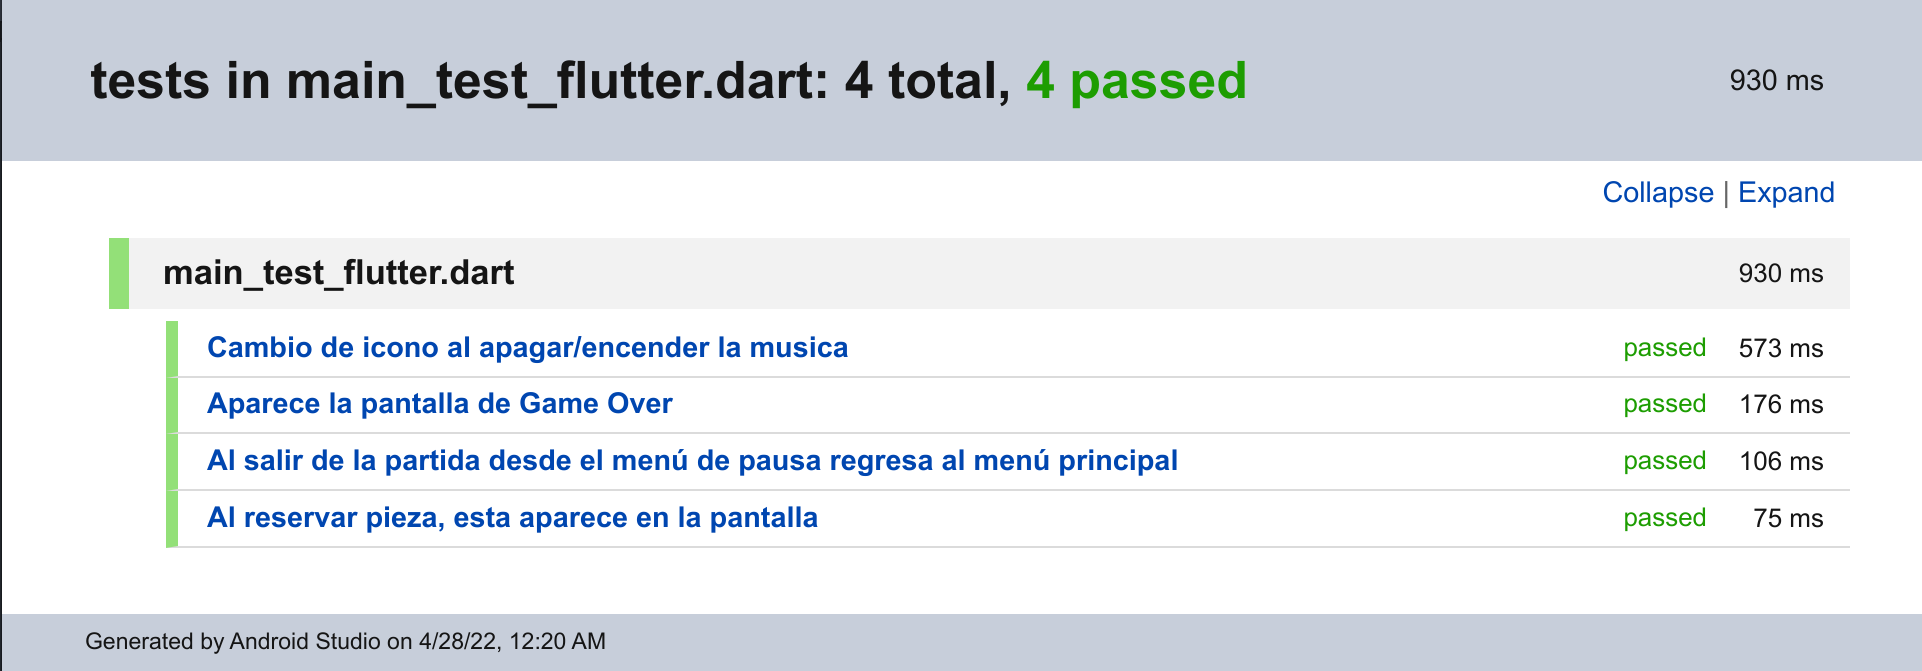
\includegraphics[width=\textwidth]{imagenes/flutter_test.png}
      \caption{Resultado de los tests de componentes/widgets}
\end{figure}

\end{document}
